\documentclass{jabstract}

\jtitle{タイトルtext\\長い場合は改行で調整}
\jauthor{自分の名前}
\jaffiliation{情報工学分野}
\jteacher{指導教員名}

\begin{document}
\maketitle

\begin{multicols}{2}
  
\section{はじめに}
導入部。ここで研究背景などを明らかにする。これには、過去の類似研究をま
とめたり、自分の研究の新規性、有用性、あるいは着想などを記すことが多い。
多くの場合、研究の目的を示すのもここになる。

\section{最初のセクション}
研究の基礎部分などの説明は、文章の流れを考えると、ほとんどの場合この辺
のセクションに記入することになる。まずここで自分の研究の立場、基礎を明
らかにしないと、読者に対して自分の主張を伝えるのが難しくなってくる。数
式
\begin{align*}
  y &= ax^2 + bx + c\\
  z &= ax^3 + bx^2 + cy^2 + d\\
  F(\xi) &= \int^{\infty}_{-\infty}f(x)e^{-2\pi ix\xi}dx
\end{align*}
などを効果的に使う必要もあるだろう。文献の引用\cite{refinfo}も大切。

\subsection{サブセクション}
必要に応じてサブセクションを設ける。しかし、紙面も限られているので本当
にサブセクションが必要かどうかは、今一度考えてみるといいだろう。サブセ
クションにせずとも、適切に段落分けすることで、十分読みやすい文章にする
ことが可能な場合が多いはずだ。
表(表~\ref{tab:sample})や図(図~\ref{fig:sample})の使い方も重要になる。

\begin{tablehere}
  \noindent
  \parbox{\linewidth}{
    \centering
    \caption{表の挿入例}\label{tab:sample}
    \begin{tabular}{|c|c|c|}
      \hline
      & jarticle & jpreprint\\
      \hline
      一段に収まる図 & figure環境 & figurehere環境\\
      \hline
      紙幅一杯の図 & figure*環境 & figure*環境\\
      \hline
      一段に収まる表 & table環境 & tablehere環境\\
      \hline
      紙幅一杯の表 & table*環境 & table*環境\\
      \hline
    \end{tabular}
  }%
\end{tablehere}

\begin{figurehere}
  \noindent
  \parbox{\linewidth}{
    \centering
    \scalebox{0.5}{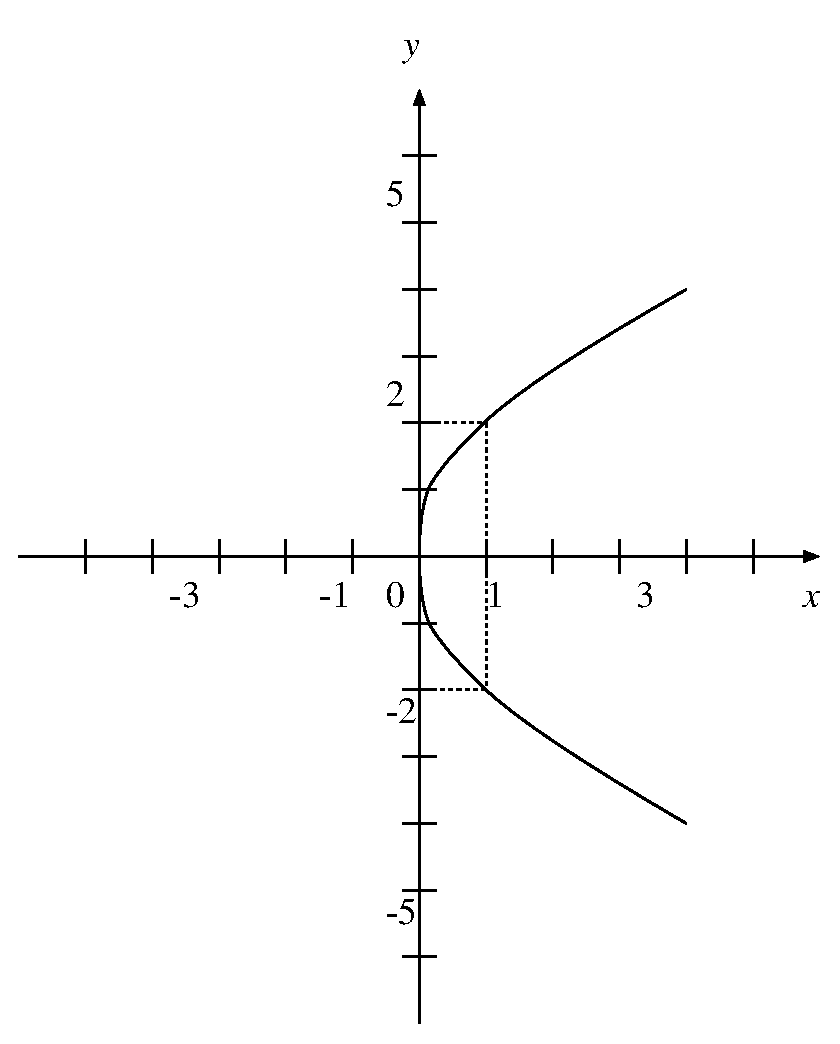
\includegraphics{sample.eps}}
    \caption{図の挿入例}\label{fig:sample}
  }%
\end{figurehere}

\section{次のセクション}
中間発表の場合は進捗状況や今後の方向性、進め方など、本発表の場合は自分
の研究の核心部分や実験などがこのあたりに来ることになるだろう。

\begin{enumerate}
\item あれ
\item これ
\item それ
\item どれ
\end{enumerate}
箇条書きは紙面を食うので、必要性を慎重に考えなければならない。

\section*{おわりに}
最後に全体をまとめ、自分の研究の成果と課題をはっきりさせることが肝心と
なる。文章全体の印象を左右することにもなるので、ここも気は抜けない。

%
% 以下に文献を書きます。
% 最後の section との間に必ず空行を開けること

{\small
\begin{thebibliography}{99}
  \bibitem{refinfo} 著者, タイトル. 書誌情報, 2025.
\end{thebibliography}
}

\end{multicols}

\end{document}
